% =============================================================================
%  INF6103 — Cybersécurité des Infrastructures Critiques
%  TP 2 : Scénario d'intrusion contre les systèmes de contrôle industriels
%  Rapport de pentest
%  Compilation : latexmk -pdf rapport.tex   (ou : make)
% =============================================================================
\documentclass[11pt,letterpaper]{article}

% --- Langue / encodage --------------------------------------------------------
\usepackage[T1]{fontenc}
\usepackage[utf8]{inputenc}
\usepackage[french]{babel}
\usepackage{lmodern}
\usepackage{csquotes}

% --- Mise en page -------------------------------------------------------------
\usepackage[margin=2.5cm]{geometry}
\usepackage{fancyhdr}
\usepackage{titlesec}
\usepackage{enumitem}
\usepackage{parskip}

% --- Tableaux / figures -------------------------------------------------------
\usepackage{graphicx}
\graphicspath{{figures/}}
\usepackage{booktabs}
\usepackage{tabularx}
\usepackage{longtable}
\usepackage{array}
\usepackage{caption}
\usepackage{subcaption}
\usepackage{float}
\usepackage{multirow}
\usepackage{threeparttable}

% --- Code / couleurs / liens --------------------------------------------------
\usepackage{xcolor}
\usepackage{listings}
\usepackage{siunitx}
\sisetup{locale=FR}
\usepackage[hidelinks]{hyperref}
\usepackage[nameinlink]{cleveref}

% --- Informations du rapport --------------------------------------------------
\newcommand{\cours}{INF6103 : Cybersécurité des Infrastructures Critiques}
\newcommand{\tptitre}{TP 2 : Scénario d'intrusion contre les systèmes de contrôle industriels}
\newcommand{\session}{Automne 2026}
\newcommand{\equipe}{Équipe XX}
\newcommand{\remise}{\today}

% Adresse de la VM (à adapter)
\newcommand{\ipvm}{\texttt{ip\_vm}}

% --- En-têtes -----------------------------------------------------------------
\pagestyle{fancy}
\fancyhf{}
\fancyhead[L]{\small \cours}
\fancyhead[R]{\small \session}
\fancyfoot[C]{\thepage}
\setlength{\headheight}{14pt}

% --- Style des listings -------------------------------------------------------
\definecolor{codebg}{HTML}{F5F5F5}
\definecolor{codecomment}{HTML}{6A737D}
\definecolor{codekw}{HTML}{005CC5}
\definecolor{codestr}{HTML}{22863A}

\lstdefinestyle{base}{
  backgroundcolor=\color{codebg},
  basicstyle=\ttfamily\footnotesize,
  keywordstyle=\color{codekw}\bfseries,
  commentstyle=\color{codecomment}\itshape,
  stringstyle=\color{codestr},
  breaklines=true,
  breakatwhitespace=false,
  columns=fullflexible,
  keepspaces=true,
  showstringspaces=false,
  frame=single,
  rulecolor=\color{black!20},
  framesep=4pt,
  xleftmargin=6pt,
  xrightmargin=6pt,
  numbers=none,
  captionpos=b,
  literate={é}{{\'e}}1 {è}{{\`e}}1 {à}{{\`a}}1 {ç}{{\c{c}}}1
           {ê}{{\^e}}1 {ô}{{\^o}}1 {É}{{\'E}}1 {ù}{{\`u}}1
           {î}{{\^i}}1 {â}{{\^a}}1
}
\lstdefinestyle{shell}{style=base, language=bash}
\lstdefinestyle{py}{style=base, language=Python, numbers=left,
  numberstyle=\tiny\color{codecomment}}
\lstdefinestyle{output}{style=base, backgroundcolor=\color{white}}
\lstset{style=base}
\renewcommand{\lstlistingname}{Listing}
\renewcommand{\lstlistlistingname}{Liste des listings}

% --- Commandes utilitaires ----------------------------------------------------
% Encadré « Question » rappelant l'énoncé
\newcommand{\question}[2]{%
  \par\noindent\fcolorbox{black!25}{black!4}{%
    \parbox{\dimexpr\linewidth-2\fboxsep-2\fboxrule}{%
      \small\textbf{Question #1} --- \emph{#2}}}\par\medskip}
% Marqueur de contenu à compléter
\newcommand{\todo}[1]{\textcolor{red}{\textbf{[À FAIRE : #1]}}}

% =============================================================================
\begin{document}

% --- Page titre ---------------------------------------------------------------
\begin{titlepage}
  \centering
  % \includegraphics[width=0.55\linewidth]{logo_poly.png}\par
  \vspace*{3cm}
  {\Large \cours\par}
  \vspace{2cm}
  \rule{\linewidth}{0.5pt}\par\vspace{0.3cm}
  {\large \tptitre\par}
  \vspace{0.1cm}\rule{\linewidth}{0.5pt}\par
  \vspace{1cm}
  {\large \textbf{Rapport de test d'intrusion}\par}
  \vspace{2cm}
  {\large \equipe\par}
  \vspace{0.5cm}
  \begin{tabular}{ll}
    Prénom Nom & Matricule \\
    Prénom Nom & Matricule \\
  \end{tabular}
  \vfill
  {\large Polytechnique Montréal\par}
  {\session\ --- Remis le \remise\par}
\end{titlepage}

\tableofcontents
\newpage

% =============================================================================
\section*{Sommaire exécutif}
\addcontentsline{toc}{section}{Sommaire exécutif}
% Résumé destiné à la direction : objectif du mandat, principales
% vulnérabilités, impact démontré, recommandations prioritaires.
\todo{Résumé du mandat, des vulnérabilités critiques et de l'impact.}

\subsection*{Périmètre et conditions}
\begin{itemize}
  \item Point d'entrée : carte RasPi (\texttt{ssh root@\ipvm{} -p 2222}).
  \item Caméra de surveillance de la cuve : \url{http://ip_vm:80}.
  \item Interface de contrôle (tunnel) : \url{http://ip_vm:9090/}.
  \item Interface de programmation du PLC (tunnel) : \url{http://ip_vm:8080/}.
\end{itemize}

% =============================================================================
\section{Reconnaissance}

\subsection{Cartographie des machines et services}
\question{1.1}{Identifiez les machines présentes sur le réseau et les services
qu'elles offrent (tableau : adresse IP, nom d'hôte, ports ouverts, services).}

La découverte a été réalisée depuis la RasPi (\texttt{192.168.95.122}) avec
\texttt{nmap -sV -p- -T4 192.168.95.0/24}. Onze hôtes actifs ont été
identifiés (tableau~\ref{tab:hosts}).

\begin{table}[H]
  \centering
  \small
  \begin{threeparttable}
  \caption{Machines et services détectés sur le réseau \texttt{192.168.95.0/24}}
  \label{tab:hosts}
  \renewcommand{\arraystretch}{1.15}
  \begin{tabular}{@{}l l r l l@{}}
    \toprule
    \textbf{Adresse IP} & \textbf{Nom d'hôte} & \multicolumn{2}{l}{\textbf{Port ouvert}} & \textbf{Service détecté (version)} \\
    \midrule
    \multirow{2}{*}{\texttt{192.168.95.2}}   & \multirow{2}{*}{\texttt{plc.scada}}
      & 502  & tcp & Modbus/TCP \\
    & & 8080 & tcp & HTTP --- Node.js (Express) \\
    \cmidrule(l){1-5}
    \multirow{2}{*}{\texttt{192.168.95.5}}   & \multirow{2}{*}{\texttt{ihm.scada}}
      & 8009 & tcp & AJP13 --- Apache JServ (protocole v1.3) \\
    & & 9090 & tcp & HTTP --- Apache Tomcat/Coyote JSP 1.1 \\
    \cmidrule(l){1-5}
    \multirow{2}{*}{\texttt{192.168.95.10}--\texttt{.15}\tnote{a}} & \multirow{2}{*}{---}
      & 502   & tcp & Modbus/TCP (\texttt{mbap?}) \\
    & & 55555 & tcp & Inconnu \\
    \cmidrule(l){1-5}
    \multirow{2}{*}{\texttt{192.168.95.101}\tnote{a}} & \multirow{2}{*}{\texttt{simulation.scada}}
      & 80    & tcp & HTTP --- Apache httpd 2.4.18 (Ubuntu) \\
    & & 55555 & tcp & Inconnu \\
    \cmidrule(l){1-5}
    \multirow{5}{*}{\texttt{192.168.95.254}} & \multirow{5}{*}{\texttt{inf6103-tp2}}
      & 22   & tcp & SSH --- OpenSSH 8.2p1 (Ubuntu) \\
    & & 80   & tcp & HTTP --- Apache httpd 2.4.18 (Ubuntu) \\
    & & 2222 & tcp & SSH --- OpenSSH 8.4p1 (Debian) \\
    & & 8080 & tcp & HTTP --- Node.js (Express) \\
    & & 9090 & tcp & HTTP --- Apache Tomcat/Coyote JSP 1.1 \\
    \cmidrule(l){1-5}
    \texttt{192.168.95.122} & \texttt{2e66cc4cb86d}\tnote{b}
      & 22   & tcp & SSH --- OpenSSH 8.4p1 (Debian) \\
    \bottomrule
  \end{tabular}
  \begin{tablenotes}\footnotesize
    \item[a] Les adresses \texttt{.10} à \texttt{.15} et \texttt{.101}
      partagent la même adresse MAC (\texttt{02:42:C0:A8:5F:65}) : il s'agit
      d'une seule machine possédant plusieurs adresses IP.
    \item[b] Notre point d'entrée (RasPi).
  \end{tablenotes}
  \end{threeparttable}
\end{table}

\subsection{Architecture réseau et modèle de Purdue}
\question{1.2}{Construisez une représentation de l'architecture du réseau
industriel. Positionnez les actifs observés dans les niveaux appropriés du
modèle de Purdue. Justifiez chaque positionnement à partir d'éléments
observables.}

La figure~\ref{fig:purdue} présente l'architecture du réseau industriel
reconstituée à partir de la reconnaissance, avec chaque actif positionné dans
le niveau correspondant du modèle de Purdue.

\begin{figure}[H]
  \centering
  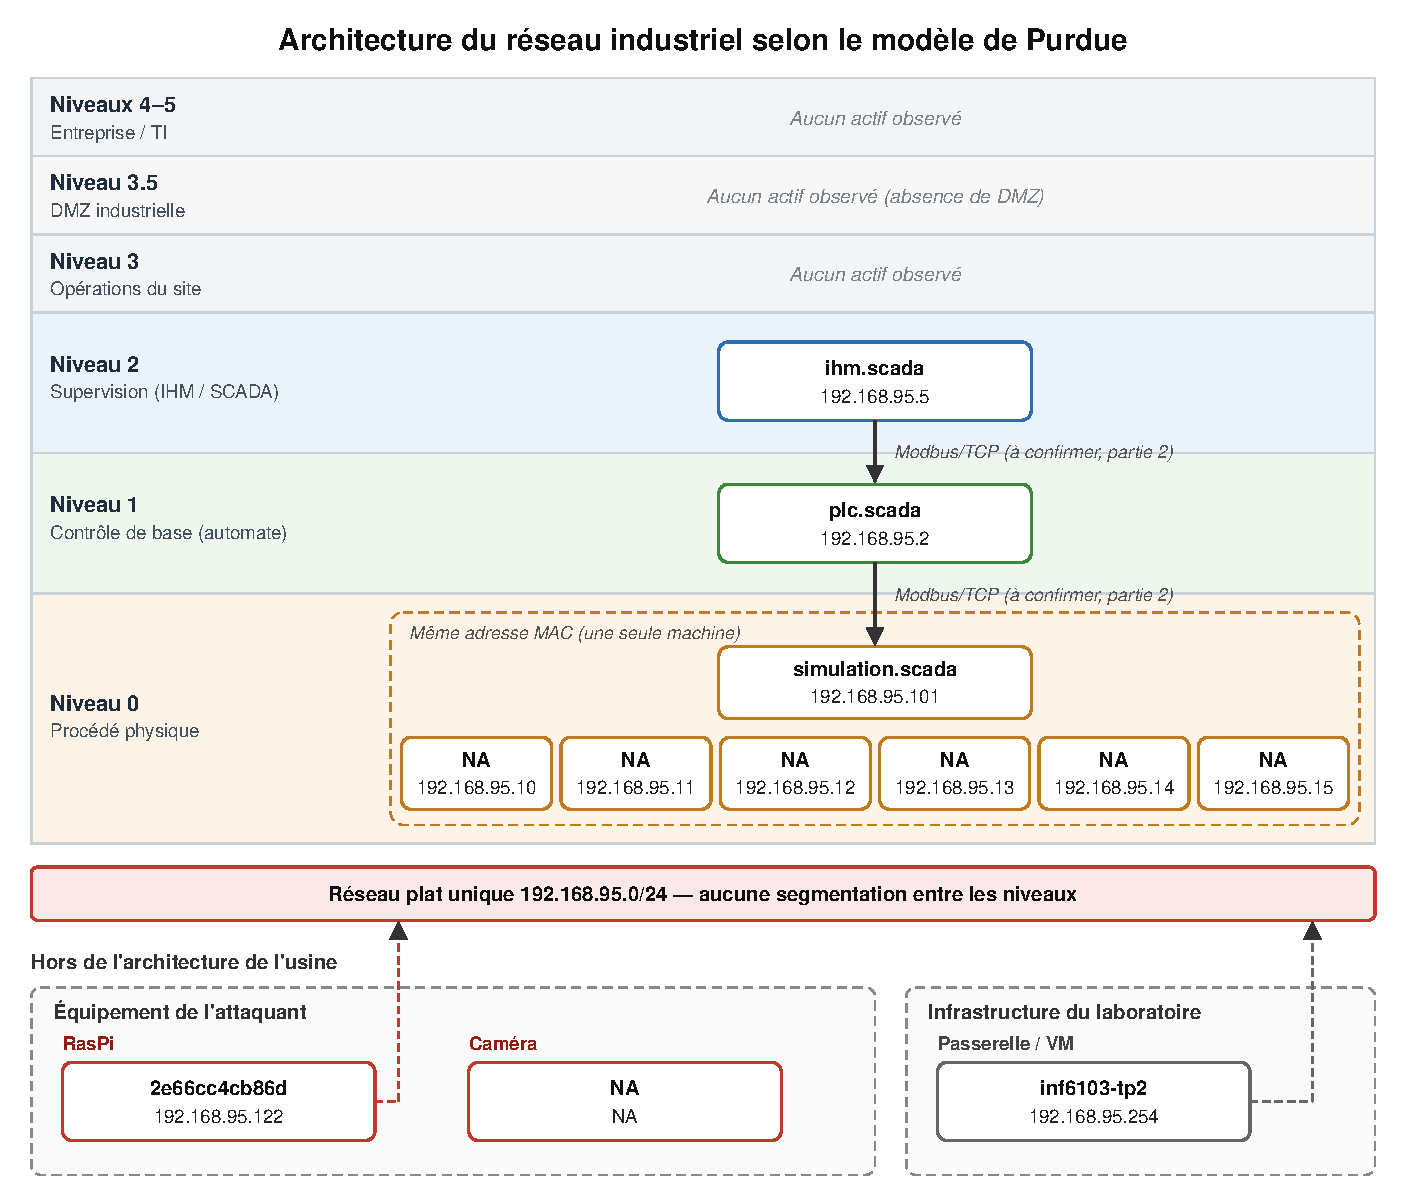
\includegraphics[width=\linewidth]{architecture_purdue.pdf}
  \caption{Architecture du réseau industriel selon le modèle de Purdue}
  \label{fig:purdue}
\end{figure}
Le positionnment sur l'échelle de Purdue repose sur trois types d'informations
observées:
\begin{enumerate}
  \item Les protocoles exposés
  \item Les noms d'hôte (scan \texttt{nmap -Sv}) 
  \item Les adresses MAC relevées lors du scan
\end{enumerate}

\textbf{Niveau 0 - Procédé physique}: simulation.scada (192.168.95.101) et 192.168.95.10-15
Les six adresses exposent un serveur Modbus/TCP (port 502) et rien d'autre 
d'après notre scan. Elles partagent toutes la même adresse MAC. Le nom d'hôte
décrit explicitement le rôle de simulation de processus physique.

\textbf{Niveau 1 - Contrôle de base}: plc.scada (192.168.95.2)
L'hôte expose un serveur Modbus/TCP, un protocole par lequel un PLC
peut être lu et commandé par un superviseur. Il expose par contre 
aussi une application Node.js/Express au port 8080. De plus 
il public la même bannière que le port 8080 publié par la VM décrit 
dans l'énoncé comme une interface de contrôle de PLC. Finalement
son nom d'hôte indique explicitement qu'il sagirait d'un PLC. Sous
toute réserve on peut poser l'hypothèse qu'il sert de lien entre le niveau
2 de supervision et les processus physiques et leurs équipements (actuators,
sensors) au niveau 0.

\textbf{Niveau 2 - Supervision}: ihm.scada (192.168.95.5)
Cet hôte ne publie aucun port de type Modbus contrairement aux
précédents. Il publie cependant le port 9090 qui selon nmap
serait un serveur Apache Tomcat/Coyote. Il présente d'ailleurs
la même bannière que le port 9090 publié par la VM décrit dans
l'énoncé comme l'interface de contrôle du système industriel.
Il y aussi le port 8009 (AJP13), probablemen une erreur de configuration
puisque ce dernier est destiné à la connexion interne avec Tomcat.

\textbf{Niveau 3-4-5}: Nous n'avons rien observé à ces niveaux.

Hors de l'architecture il y a la carte RasPi et la caméra qui sont des
machines de l'attaquant et ne prennent donc pas place dans le modèle de Purdue.

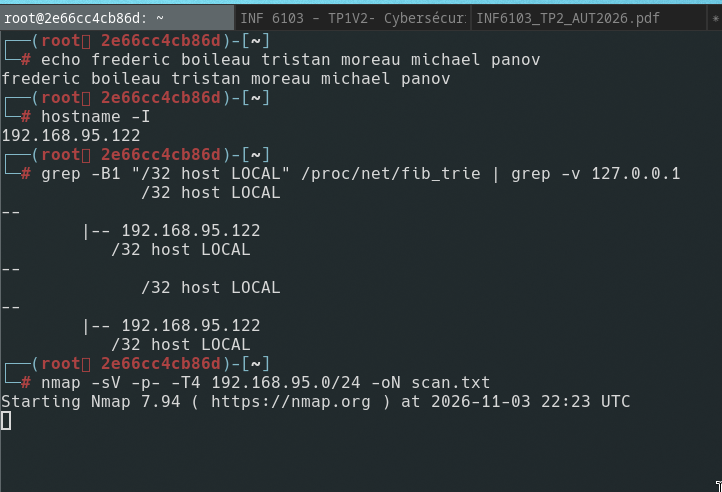
\includegraphics[width=\textwidth]{images/recon.png}

\clearpage
\subsection{Accès à la page d'authentification}
\question{1.3}{Accédez à la page d'authentification de l'interface de contrôle
du système industriel.}

L'interface de contrôle est hébergée par \texttt{ihm.scada}
(\texttt{192.168.95.5:9090}), nous établissons d'abord
un tunnel ssh pour faire un port fowward local.
\begin{lstlisting}[style=shell, caption={Tunnel SSH vers l'IHM à travers la RasPi}, label={lst:tunnel}]
ssh -N -f -L 8090:192.168.95.5:9090 root@192.168.56.101 -p 2222
\end{lstlisting}
Nous utilisons l'outil \texttt{gobuster} pour énumérer les path
disponibles sur le serveur étant donné que la racine donne
juste la page par défaut de Tomcat.
\begin{lstlisting}[style=shell, caption={Énumération des chemins du serveur Tomcat}, label={lst:gobuster}]
gobuster dir -u http://localhost:8090/ -w common.txt
\end{lstlisting}
Nous trouvons le chemin intéressant \texttt{host-manager} et
y accédons avec notre navigateur. Nous sommes par la suite
interrogé par un dialogue HTTP basic auth. Voir capture
pour tout le processus à la figure \ref{fig:gobuster}

\begin{figure}[H]
  \centering
  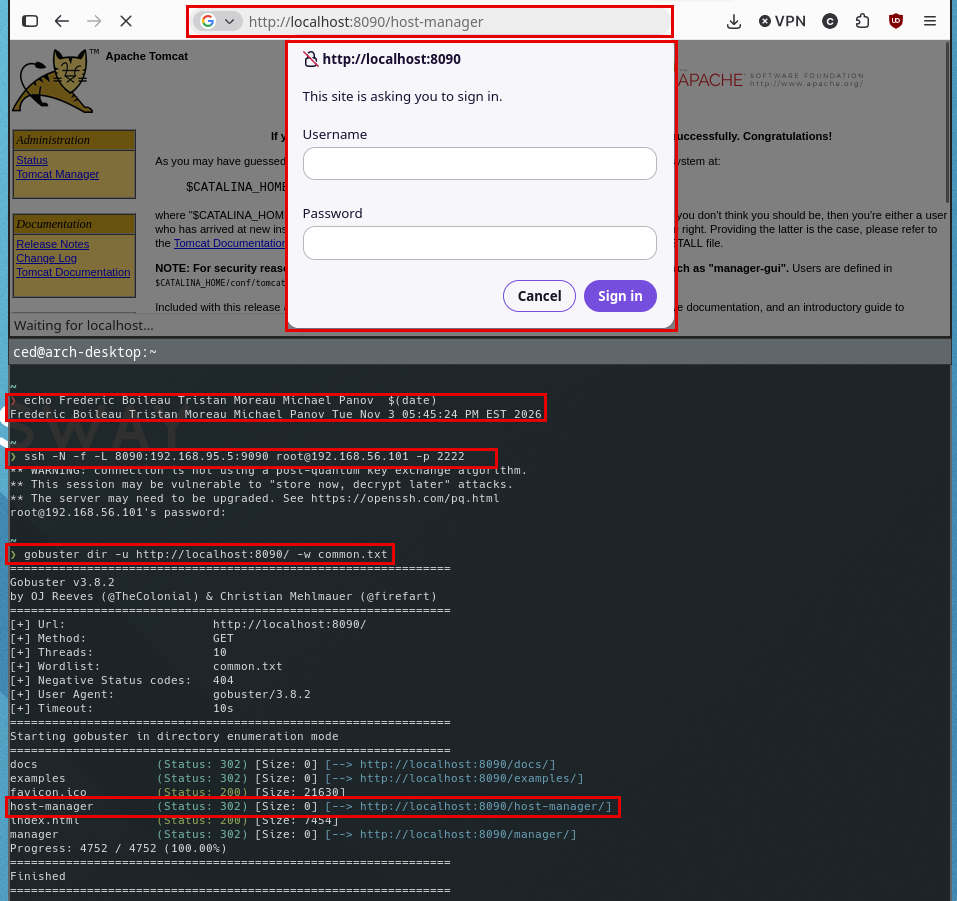
\includegraphics[width=\linewidth]{images/adminpage_annotee.png}
  \caption{Tunnel SSH, énumération des chemins et authentification de
  \texttt{/host-manager}}
  \label{fig:gobuster}
\end{figure}

\clearpage
\subsection{Tentative d'authentification}
\question{1.4}{Tentez une authentification avec les identifiants
\texttt{username=admin} \& \texttt{password=admin}.}

\begin{figure}[H]
  \centering
  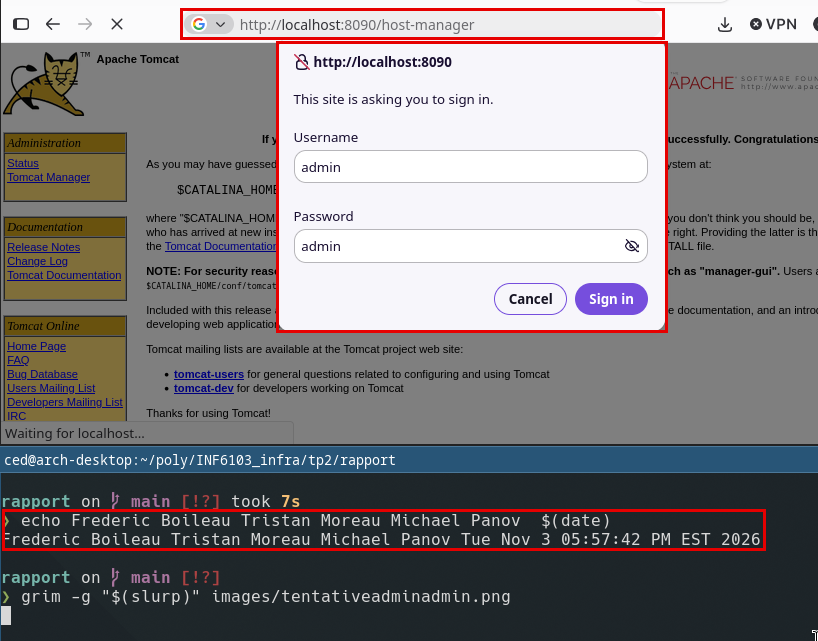
\includegraphics[width=\linewidth]{images/tentativeadminadmin_annotee.png}
  \caption{Tentative d'authentification avec \texttt{admin}/\texttt{admin}}
  \label{fig:adminadmin}
\end{figure}



\end{document}
